%===================================================================================
% JORNADA CIENTÍFICA ESTUDIANTIL - MATCOM, UH
%===================================================================================
% Esta plantilla ha sido diseñada para ser usada en los artículos de la
% Jornada Científica Estudiantil, MatCom.
%
% Por favor, siga las instrucciones de esta plantilla y rellene en las secciones
% correspondientes.
%
% NOTA: Necesitará el archivo 'jcematcom.sty' en la misma carpeta donde esté este
%       archivo para poder utilizar esta plantila.
%===================================================================================



%===================================================================================
% PREÁMBULO
%-----------------------------------------------------------------------------------
\documentclass[a4paper,10pt,twocolumn]{article}

%===================================================================================
% Paquetes
%-----------------------------------------------------------------------------------
\usepackage{amsmath}
\usepackage{amsfonts}
\usepackage{amssymb}
\usepackage{jcematcom}
\usepackage[utf8]{inputenc}
\usepackage{listings}
\usepackage[pdftex]{hyperref}
\usepackage{graphicx}
%-----------------------------------------------------------------------------------
% Configuración
%-----------------------------------------------------------------------------------
\hypersetup{colorlinks,%
	    citecolor=black,%
	    filecolor=black,%
	    linkcolor=black,%
	    urlcolor=blue}

\graphicspath{ {./images/} }
%===================================================================================



%===================================================================================
% Presentacion
%-----------------------------------------------------------------------------------
% Título
%-----------------------------------------------------------------------------------
\title{Estadística\\Clase Práctica 9\\Ejercicio 1}

%-----------------------------------------------------------------------------------
% Autores
%-----------------------------------------------------------------------------------
\author{\\
\name Carlos Bermudez Porto \email \href{mailto:c.bermudez@estudiantes.matcom.uh.cu}{c.bermudez@estudiantes.matcom.uh.cu}
	\\ \addr Grupo C412 \AND
\name Leynier Gutiérrez González \email \href{mailto:l.gutierrez@estudiantes.matcom.uh.cu}{l.gutierrez@estudiantes.matcom.uh.cu}
  \\ \addr Grupo C412 \AND
\name Tony Raúl Blanco Fernández \email \href{mailto:t.blanco@estudiantes.matcom.uh.cu}{t.blanco@estudiantes.matcom.uh.cu}
  \\ \addr Grupo C411}

%-----------------------------------------------------------------------------------
% Tutores
%-----------------------------------------------------------------------------------
\tutors{\\
Lic. Dalia Diaz Sistachs, \emph{Departamento de Matemática Aplicada}}

%-----------------------------------------------------------------------------------
% Headings
%-----------------------------------------------------------------------------------
\jcematcomheading{\the\year}{1-\pageref{end}}{C. Bermudez, L. Gutiérrez, T. Blanco}

%-----------------------------------------------------------------------------------
\ShortHeadings{Proyecto Fase 2 de Estadística}{Autores}
%===================================================================================



%===================================================================================
% DOCUMENTO
%-----------------------------------------------------------------------------------
\begin{document}

%-----------------------------------------------------------------------------------
% NO BORRAR ESTA LINEA!
%-----------------------------------------------------------------------------------
\twocolumn[
%-----------------------------------------------------------------------------------

\maketitle

%===================================================================================
% Resumen y Abstract
%-----------------------------------------------------------------------------------
\selectlanguage{spanish} % Para producir el documento en Español

%-----------------------------------------------------------------------------------
% Resumen en Español
%-----------------------------------------------------------------------------------
% \begin{abstract}

% 	El Resumen en Español debe constar de $100$ a $200$ palabras y presentar de forma
% 	clara y concisa el contenido fundamental del artículo.

% \end{abstract}

%-----------------------------------------------------------------------------------
% English Abstract
%-----------------------------------------------------------------------------------
% \vspace{0.5cm}

% \begin{enabstract}

%   The English Abstract must have have $100$ to $200$ words, and present in a clear
%   and concise form the essentials of the article content.

% \end{enabstract}

%-----------------------------------------------------------------------------------
% Palabras clave
%-----------------------------------------------------------------------------------
\begin{keywords}
	k-means,
	acp,
	clusters,
	d-tree
\end{keywords}

%-----------------------------------------------------------------------------------
% Temas
%-----------------------------------------------------------------------------------
\begin{topics}
	Estadística, Análisis de Componentes Principales, Técnicas de Clasificación
\end{topics}


%-----------------------------------------------------------------------------------
% NO BORRAR ESTAS LINEAS!
%-----------------------------------------------------------------------------------
\vspace{0.8cm}
]
%-----------------------------------------------------------------------------------


%===================================================================================

%===================================================================================
% Introducción
%-----------------------------------------------------------------------------------
\section{Introducción}\label{sec:intro}
%-----------------------------------------------------------------------------------

El siguiente trabajo corresponde a la realización del ejercicio 1 de la clase práctica 9 de los autores como evaluación de la asignatura de Estadística de la carrera de Ciencia de la Computación de la Facultad de Matemática y Computación de la Universidad de La Habana.

Los datos utilizados para el trabajo son sacados de un estudio en adolecentes con desórdenes alimenticios conocidos con el objetivo de encontrar una sintomatología estandar para comportamientos de anorexia y bulimia. En cada observación las pacientes fueron valoradas en síntomas diferentes.

Se decidió eliminar la columna $number$ pues en si esta es equivalente a un identificador del paciente y no aporta informacion real al problema.

En las pruebas de hipótesis se asumió un nivel de significación del $5\%$, por tanto, fue posible aceptar las hipótesis nulas con una probabilidad de error menor o igual a $0.05$.

\section{Análisis de Correlación}\label{sec:ana_cor}

% Se analizó la correlación entre las diferentes variables utilizando las funciones $symnum$ (Fig. \ref{fig:symnum}) y $pairs$ (Fig. \ref{fig:pairs}).

Se analizó la correlación entre las diferentes variables utilizando la función $symnum$ (Fig. \ref{fig:symnum})).


\begin{figure}[htb]%
	\begin{center}
		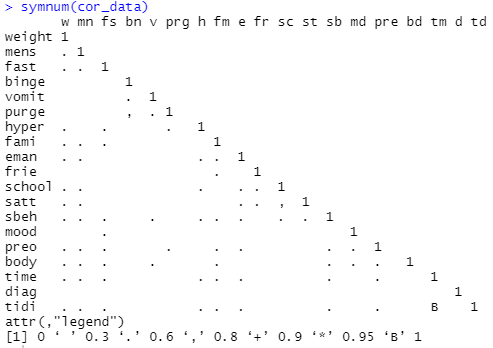
\includegraphics[width=\linewidth]{symnum}
	\end{center}
	\caption{Resultado de la función $symnum$ \label{fig:symnum}}%
\end{figure}

% \begin{figure}[htb]%
% 	\begin{center}
% 		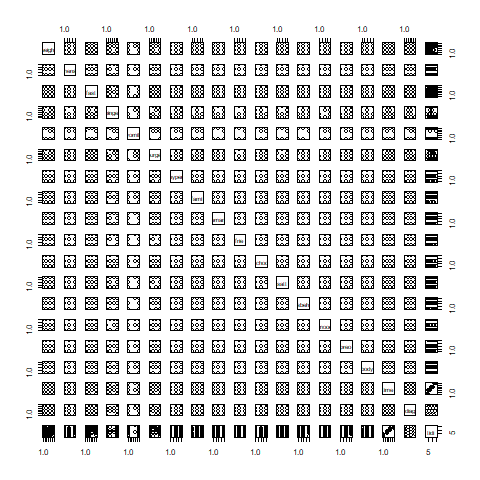
\includegraphics[width=\linewidth]{pairs}
% 	\end{center}
% 	\caption{Resultado de la función $pairs$ \label{fig:pairs}}%
% \end{figure}

Como se pudo observar casi todas las variables estan poco correlacionadas con el resto, debido a la abundancia de '.'  y  ' '. Existe solo un caso de variables muy correlacionadas, la variable $tidi$ y $time$. De cualquier forma la reduccion de dimensión es factible.

\section{Análisis de Componentes Principales}\label{sec:acp}

% Se analizaron todas las variables pues no serán utilizadas para una regresión. (Fig. \ref{fig:variances} y \ref{fig:acp})

Se analizaron todas las variables pues no serán utilizadas para una regresión. (Fig. \ref{fig:acp})

% \begin{figure}[htb]%
% 	\begin{center}
% 		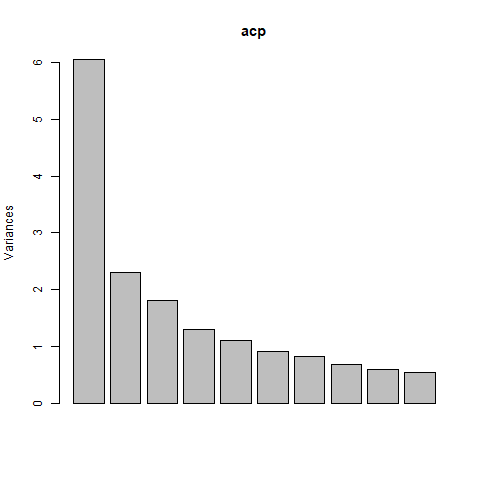
\includegraphics[width=\linewidth]{variances}
% 	\end{center}
% 	\caption{Resultado gráfico del análisis de las componentes principales \label{fig:variances}}%
% \end{figure}

\begin{figure}[htb]%
	\begin{center}
		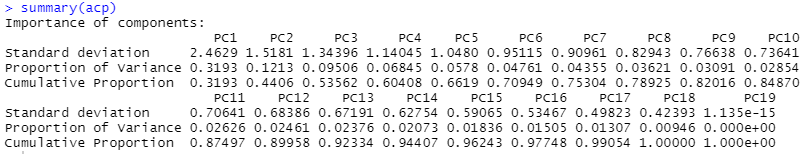
\includegraphics[width=\linewidth]{acp}
	\end{center}
	\caption{Resultado del análisis de las componentes principales \label{fig:acp}}%
\end{figure}

Despues de analizados los valores propios se pudo notar que usando el criterio del porcentaje o el criterio de Kaiser (para valores propios mayores que 1) era posible usar entre $5$ y $6$ componentes principales. Por simplicidad se utilizaron $5$.

\subsection{Descripción de las Componentes}\label{sec:desc_comp}

\begin{figure}[htb]%
	\begin{center}
		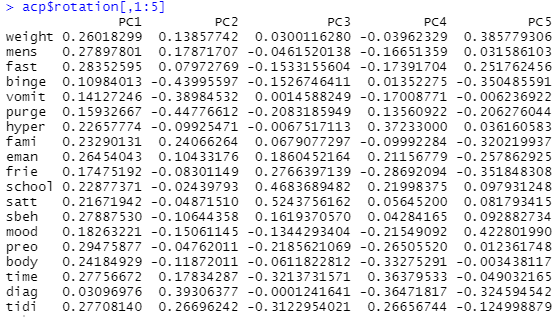
\includegraphics[width=\linewidth]{rotation}
	\end{center}
	\caption{Descripción de las Componentes \label{fig:rotation}}%
\end{figure}

\begin{itemize}
	\item \textbf{PC1:} Para la primera componente encontramos que exite una precencia de las pacientes con alto peso, (aparece menstruacion pero no se explicarla), que ademas tienen una alta restriccion de comida, que ademas purgan(viene de la traduccion de purge en este contxto qu no domino) despues de ingerir alimentos, con hiperactividad, buenas relaciones con familiares y amigos, alta emancipacion de sus familias, (desconozco school para que sera), buena actitud y comportamiento sexual, con buen estado de animo, muy preocupadas por su alimentacion y peso corporal, con mucha percepcion de su cuerpo, (por ultimo time y tidi tambien pero no logro interpretar a que se refieren).
	
	\item \textbf{PC2:} La segunda componente esta conformada por un grupo de pacientes con caracteristicas como pocos atracones, poca precensia de vomitos, que purgan(ver anterior referencia) poco las comidas, con buenas relaciones familiares, pero que fueron diagnosticadas con la enfermedad(asumimos q alto es q sea mas grave), (tambien esta tidi pero no tengo interpretacion).
	
	\item \textbf{PC3:} La tercera componente presenta pacientes con caracteristicas como buenas relaciones con amigos, (alto school pero sin interpretacion), buena actitud sexual, (poco time y poco tidi).
	
	\item \textbf{PC4:} La cuarta componente muestra pacientes con alta hiperactividad, con emancipacion de sus familias, sin buenas realciones con sus amigos, (school alto sin interpretacion), desanimadas, con poco preocupacion por su peso y alimentacion, poca percepcion de su cuerpo, (altos time y tidi sin interpretacion), y con poca precensia de la enfermedad.
	
	\item \textbf{PC5:} La quinta componenete se caracterisa por tener presencia de pacientes con alto peso corporal, pocos atracones, malas relaciones familiares, malas relaciones con amistades, buen estado de animo y sin presencia de la enfermedad.
\end{itemize}

Ahora veamos como se agrupan estos datos usando cluster jerarquicos, kmeans y arbol de decisión.

\section{Clusters}\label{sec:clusters}

\begin{itemize}
	\item Con $4$ clusters se puede observar (Fib. \ref{fig:hier_cluster_4_euclidean}) que se forman grandes grupos pero que aun pudiera seguir particionandoce.
	\item Lo haremos para $5$ clusters (Fib. \ref{fig:hier_cluster_5_euclidean}). Esto a partir de la observacion del dendrograma con $4$ clusters. Además intuitivamente por la cantidad de componentes principales que tomamos.
	\item Con $6$ clusters (Fib. \ref{fig:hier_cluster_6_euclidean}) no se nota un gran cambio con respecto a los grupos formados para $5$ clusters por eso trabajaremos con $5$ como principal cantidad de conjuntos.
\end{itemize}

Lo que si es cierto es que existen una gran cantidad de subtipos y por ende muchos grupos pequeños.

\section{K-means}\label{sec:kmeans}

\begin{itemize}
	\item Comprobando para 4 (Fib. \ref{fig:kmeans_cluster_4}) la similitude entre elementos del mismo grupo es del $36\%$, la cual es bien baja. Las cantidades en los grupos son de $67$, $19$, $88$ y $43$.
	\item De igual forma usaremos 5 (Fib. \ref{fig:kmeans_cluster_5}) grupos como medidor principal. La similitud es del $41\%$, la cual igualmente no es tan buena. Las cantidades son $28$, $85$, $47$, $19$ y $38$.
	\item Para 6 (Fib. \ref{fig:kmeans_cluster_6}) esta similitud alcanza el $44.3\%$. La diferencia no es substancial con respecto a $5$. Las cantidades son $37$, $71$, $27$, $18$, $36$ y $28$. De esas cantidades si se puede observar que al menos los elementos estan mejor distribuidos que con las cantidades de clusteres anteriores.
\end{itemize}

\section{Árbol de Decisión}\label{sec:dtree}

Analisaremos el arbol de decision (Fig. \ref{fig:d_tree_cluster_diag_class_8}) formado para la variable diag(Diagnostico) utilizando un metodo CART de clasificacion. En este caso alcanzamos un $40\%$ de error aproximadamente. El arbol es posible de construir pero no tienve mucho valor predictivo debido al alto error en un contexto en el cual este no es permisible.

\section{Referencias}\label{sec:ref}

\begin{itemize}
	\item Conferencia 5 - Corelacion
	\item Conferencia 6 - Regresion Lineal Simple
	\item Conferencia 7 - Regresion Lineal Multiple
	\item Conferencia 8 - ANOVA
	\item Conferencia 10 - Cluster, Arboles de Decisión
\end{itemize}

\newpage

\section{Anexos}\label{sec:anexos}

\begin{figure}[htb]%
	\begin{center}
		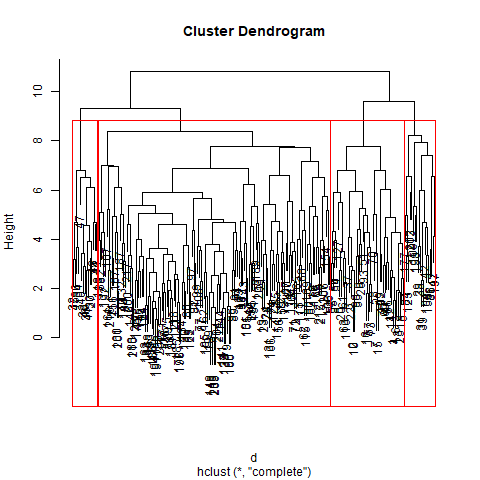
\includegraphics[width=\linewidth]{hier_cluster_4_euclidean}
	\end{center}
	\caption{Análisis con 4 clusters \label{fig:hier_cluster_4_euclidean}}%
\end{figure}

\begin{figure}[htb]%
	\begin{center}
		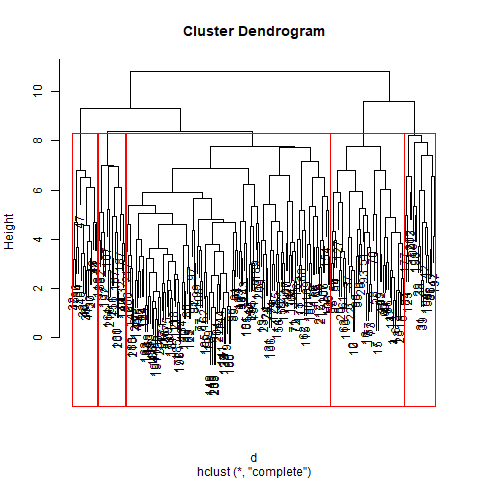
\includegraphics[width=\linewidth]{hier_cluster_5_euclidean}
	\end{center}
	\caption{Análisis con 5 clusters \label{fig:hier_cluster_5_euclidean}}%
\end{figure}

\begin{figure}[htb]%
	\begin{center}
		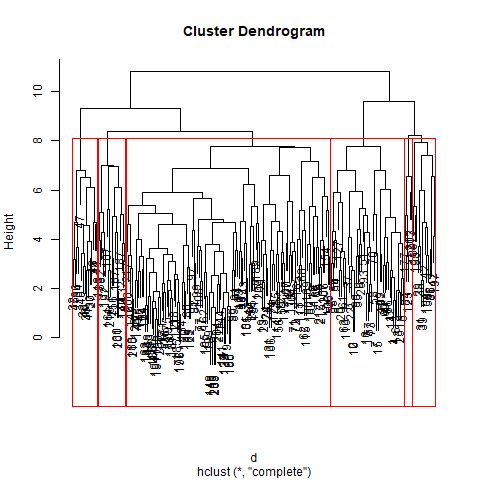
\includegraphics[width=\linewidth]{hier_cluster_6_euclidean}
	\end{center}
	\caption{Análisis con 6 clusters \label{fig:hier_cluster_6_euclidean}}%
\end{figure}

\begin{figure}[htb]%
	\begin{center}
		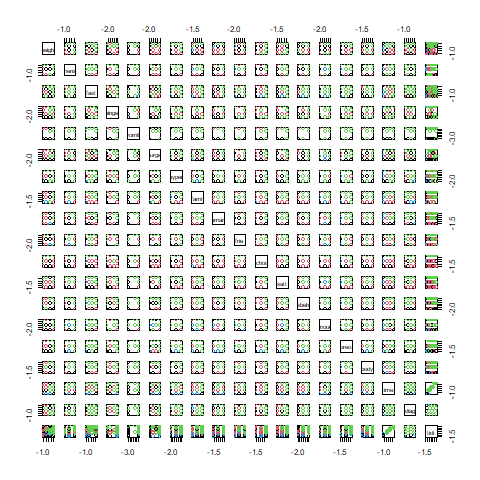
\includegraphics[width=\linewidth]{kmeans_cluster_4}
	\end{center}
	\caption{Análisis de kmeans con 4 \label{fig:kmeans_cluster_4}}%
\end{figure}

\begin{figure}[htb]%
	\begin{center}
		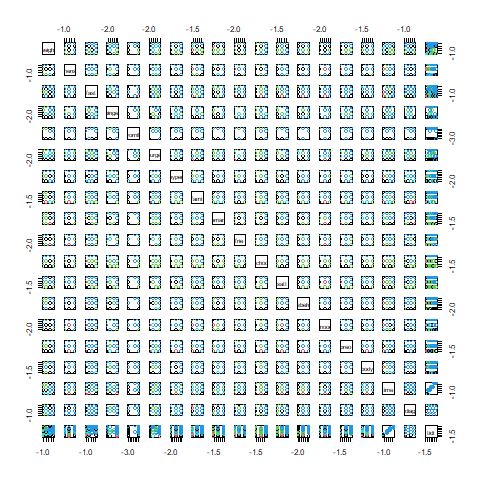
\includegraphics[width=\linewidth]{kmeans_cluster_5}
	\end{center}
	\caption{Análisis de kmeans con 5 \label{fig:kmeans_cluster_5}}%
\end{figure}

\begin{figure}[htb]%
	\begin{center}
		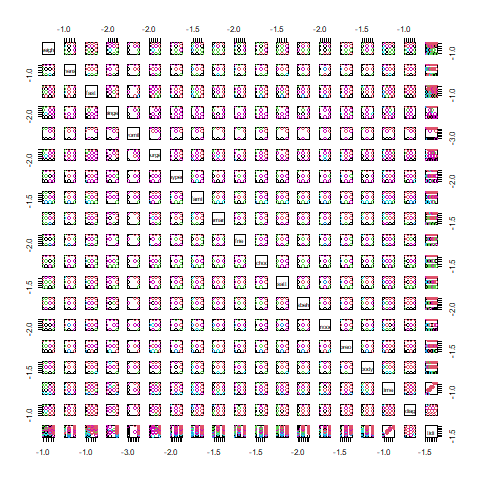
\includegraphics[width=\linewidth]{kmeans_cluster_6}
	\end{center}
	\caption{Análisis de kmeans con 6 \label{fig:kmeans_cluster_6}}%
\end{figure}

\begin{figure}[htb]%
	\begin{center}
		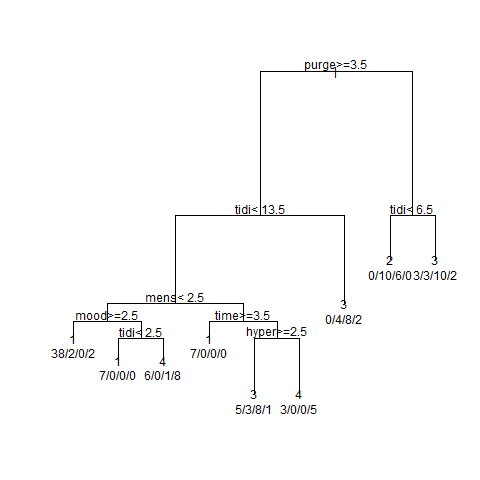
\includegraphics[width=\linewidth]{d_tree_cluster_diag_class_8}
	\end{center}
	\caption{Árbol de Decisión \label{fig:d_tree_cluster_diag_class_8}}%
\end{figure}

%-----------------------------------------------------------------------------------

\label{end}

\end{document}

%===================================================================================
